\chapter{Optimización Inteligente}
Planificación y Scheduling representa un área de gran relevancia en Inteligencia Artificial. Muchos problemas reales se modelan como problemas de P\&S.

La planificación es un proceso de deliberación que escoge y
organiza acciones anticipando sus resultados o
consecuencias.

Lo scheduling es un proceso de asignación de recursos a tareas sobre el tiempo para optimizar uno o más objetivos.

\begin{figure}[htbp]
   \centering
   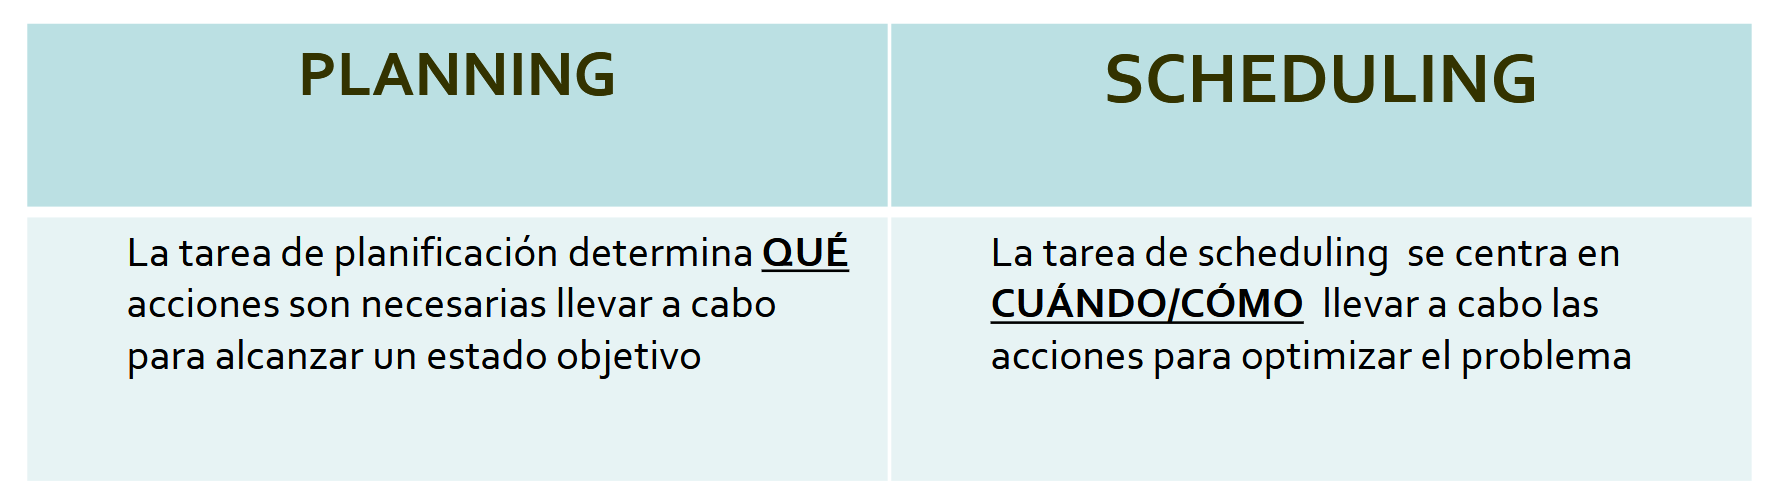
\includegraphics{images/04/PS.png}
   \caption{P\&S}
   \label{fig:04/PS}
\end{figure}
\section{Scheduling}
Un problema de scheduling consiste en organizar en el tiempo un
conjunto de actividades que compiten por el uso limitado de recursos


\subsection{JSP}
JSP stands for Job-Shop Scheduling, y es un paradigma de los problemas de scheduling es muy simple de
enunciar y muy difícil de resolver.

\begin{paracol}{2}
   \colfill
   \begin{itemize}
      \item $n$ trabajos cada uno compuesto por un conjunto ordenado de tareas
      \item $m$ maquinas donde se procesan las tareas
      \item Cada tarea debe ser procesada en una única máquina durante un tiempo determinado y en un orden prefijado;
      \item El objetivo es minimizar \textit{makespan}: instante de finalización de la última tarea
   \end{itemize}
   \colfill
   \switchcolumn

   \begin{itemize}
      \item \textbf{Datos} - $p_{ij}$ es el tiempo de proceso de la tarea i en el trabajo j;
      \item \textbf{Variables} - $st_{ij}$ es el tiempo de inicio de tarea i en el trabajo j;
      \item \textbf{Restricciones} -
      \begin{itemize}
         \item Secuential - $st_{ij} + p_{ij} \leq st_{i(j+1)}$
         \item Capacidad - $st_{ij} + p_{ij} \leq st_{kl} \bigvee st_{kl} + pkl \leq st_{ij}$
         \item Sin interrupción - $Cij = st_{ij} + p_{ij}$
      \end{itemize}
      \item \textbf{Objetivo} - Construir una ordenación de las tareas en el tiempo de manera que
      se satisfagan todas las restricciones sobre cada máquina.

      \begin{itemize}
         \item Mimimize the makespan: $C_{max} = max C_{ij}$
         \item Minimize total flow time: $C_{sum} = \sum C{i}$
         \item Minimize makespan + energy
      \end{itemize}
   \end{itemize}

\end{paracol}

\subsection{CSP - Constraint Satisfaction Problem}
{Muchos problemas pueden ser expresados mediante:\ns
\begin{itemize}
	\item Un conjunto de variables.
	\item Un dominio de interpretación (valores) para las variables.
	\item Un conjunto de restricciones entre las variables.
   \item La solución al problema es una asignación válida de valores a las variables.
\end{itemize}}

\note{Formalization omitted here}